\documentclass[../main.tex]{subfiles}

\begin{document}
    We dropped off \textit{Nantes} and \textit{Dijon} for the moment, as the \textit{3DS} scenes are not well formated. We will take care of these once we have a simple, not too time consuming, solution to read the \textit{cityGML} files: the easiest for now is to convert \textit{cityGML} to \textit{OBJ} file and write the corrspponding file handler. In consequence, We are focusing, right now, on \href{https://www.google.fr/maps/place/%C3%89lancourt/@48.7781732,1.9536264,5868m/data=!3m1!1e3!4m13!1m7!3m6!1s0x47e68370e965167b:0x705d83a4167c877c!2s%C3%89lancourt!3b1!8m2!3d48.782907!4d1.960077!3m4!1s0x47e68370e965167b:0x705d83a4167c877c!8m2!3d48.782907!4d1.960077}{\textit{Elancourt}}.\\

    We will describe fully the studied dataset used hereafter.

    \subsection{Description}

    Figure~\ref{fig::snaps} represents $.2\text{ K}m^2$ of reconstructed area that we annotated. The $3D$ buildings are obtained by \textit{Bati3D}; a home made industrialized version of~\cite{durupt2006automatic, taillandier2004automatic, taillandier2005}. Actually, the original method~\cite{taillandier2004automatic} solves a maximal clique problem equivalent to possible shapes of buildings obtained from the extracted planar primitives. The result is then adapted by applying geometric constraints. Since the clique problem is NP-complete, One solution is to reduce the search space by applying constraints early on~\cite{taillandier2005}. Another solution was to relax the constraints and aplying the RANSAC algorithm~\cite{Fischler:1981:RSC:358669.358692}.\\

    In addition to the \textit{Bati3D} outputs that we ought to qualify, we have also aquirred the corresponding \textit{DSM}s --- Figure~\ref{fig::dsm} --- and \textit{Orthoimages} --- Figure~\ref{fig::ortho}.

    \thisfloatsetup{heightadjust=object}
    \begin{figure}[H]
        \begin{minipage}[c]{\textwidth}
            \ffigbox[\FBwidth]
            {
                \begin{subfloatrow}[2]
                    \captionsetup{labelformat=brace, justification=raggedright}
                    \ffigbox[\FBwidth]
                    {
                        \includegraphics[width=.45\textwidth]{../images/raster/snapshot_1}
                    }
                    {
                        \caption{Close up snapshot of the 3D scene.}\label{fig::snap1}
                    }
                    \ffigbox[\FBwidth]
                    {
                        \includegraphics[width=.45\textwidth]{../images/raster/snapshot_2}
                    }
                    {
                        \caption{Perspective snapshot of the 3D scene.}\label{fig::snap2}
                    }
                \end{subfloatrow}
            }
            {
                \caption{\label{fig::snaps} The annotated 3D scene.}
            }
        \end{minipage}
    \end{figure}

    \thisfloatsetup{heightadjust=object}
    \begin{figure}[H]
        \ffigbox[\FBwidth]
        {
            \begin{subfloatrow}[2]
                \ffigbox[\FBwidth]
                {
                    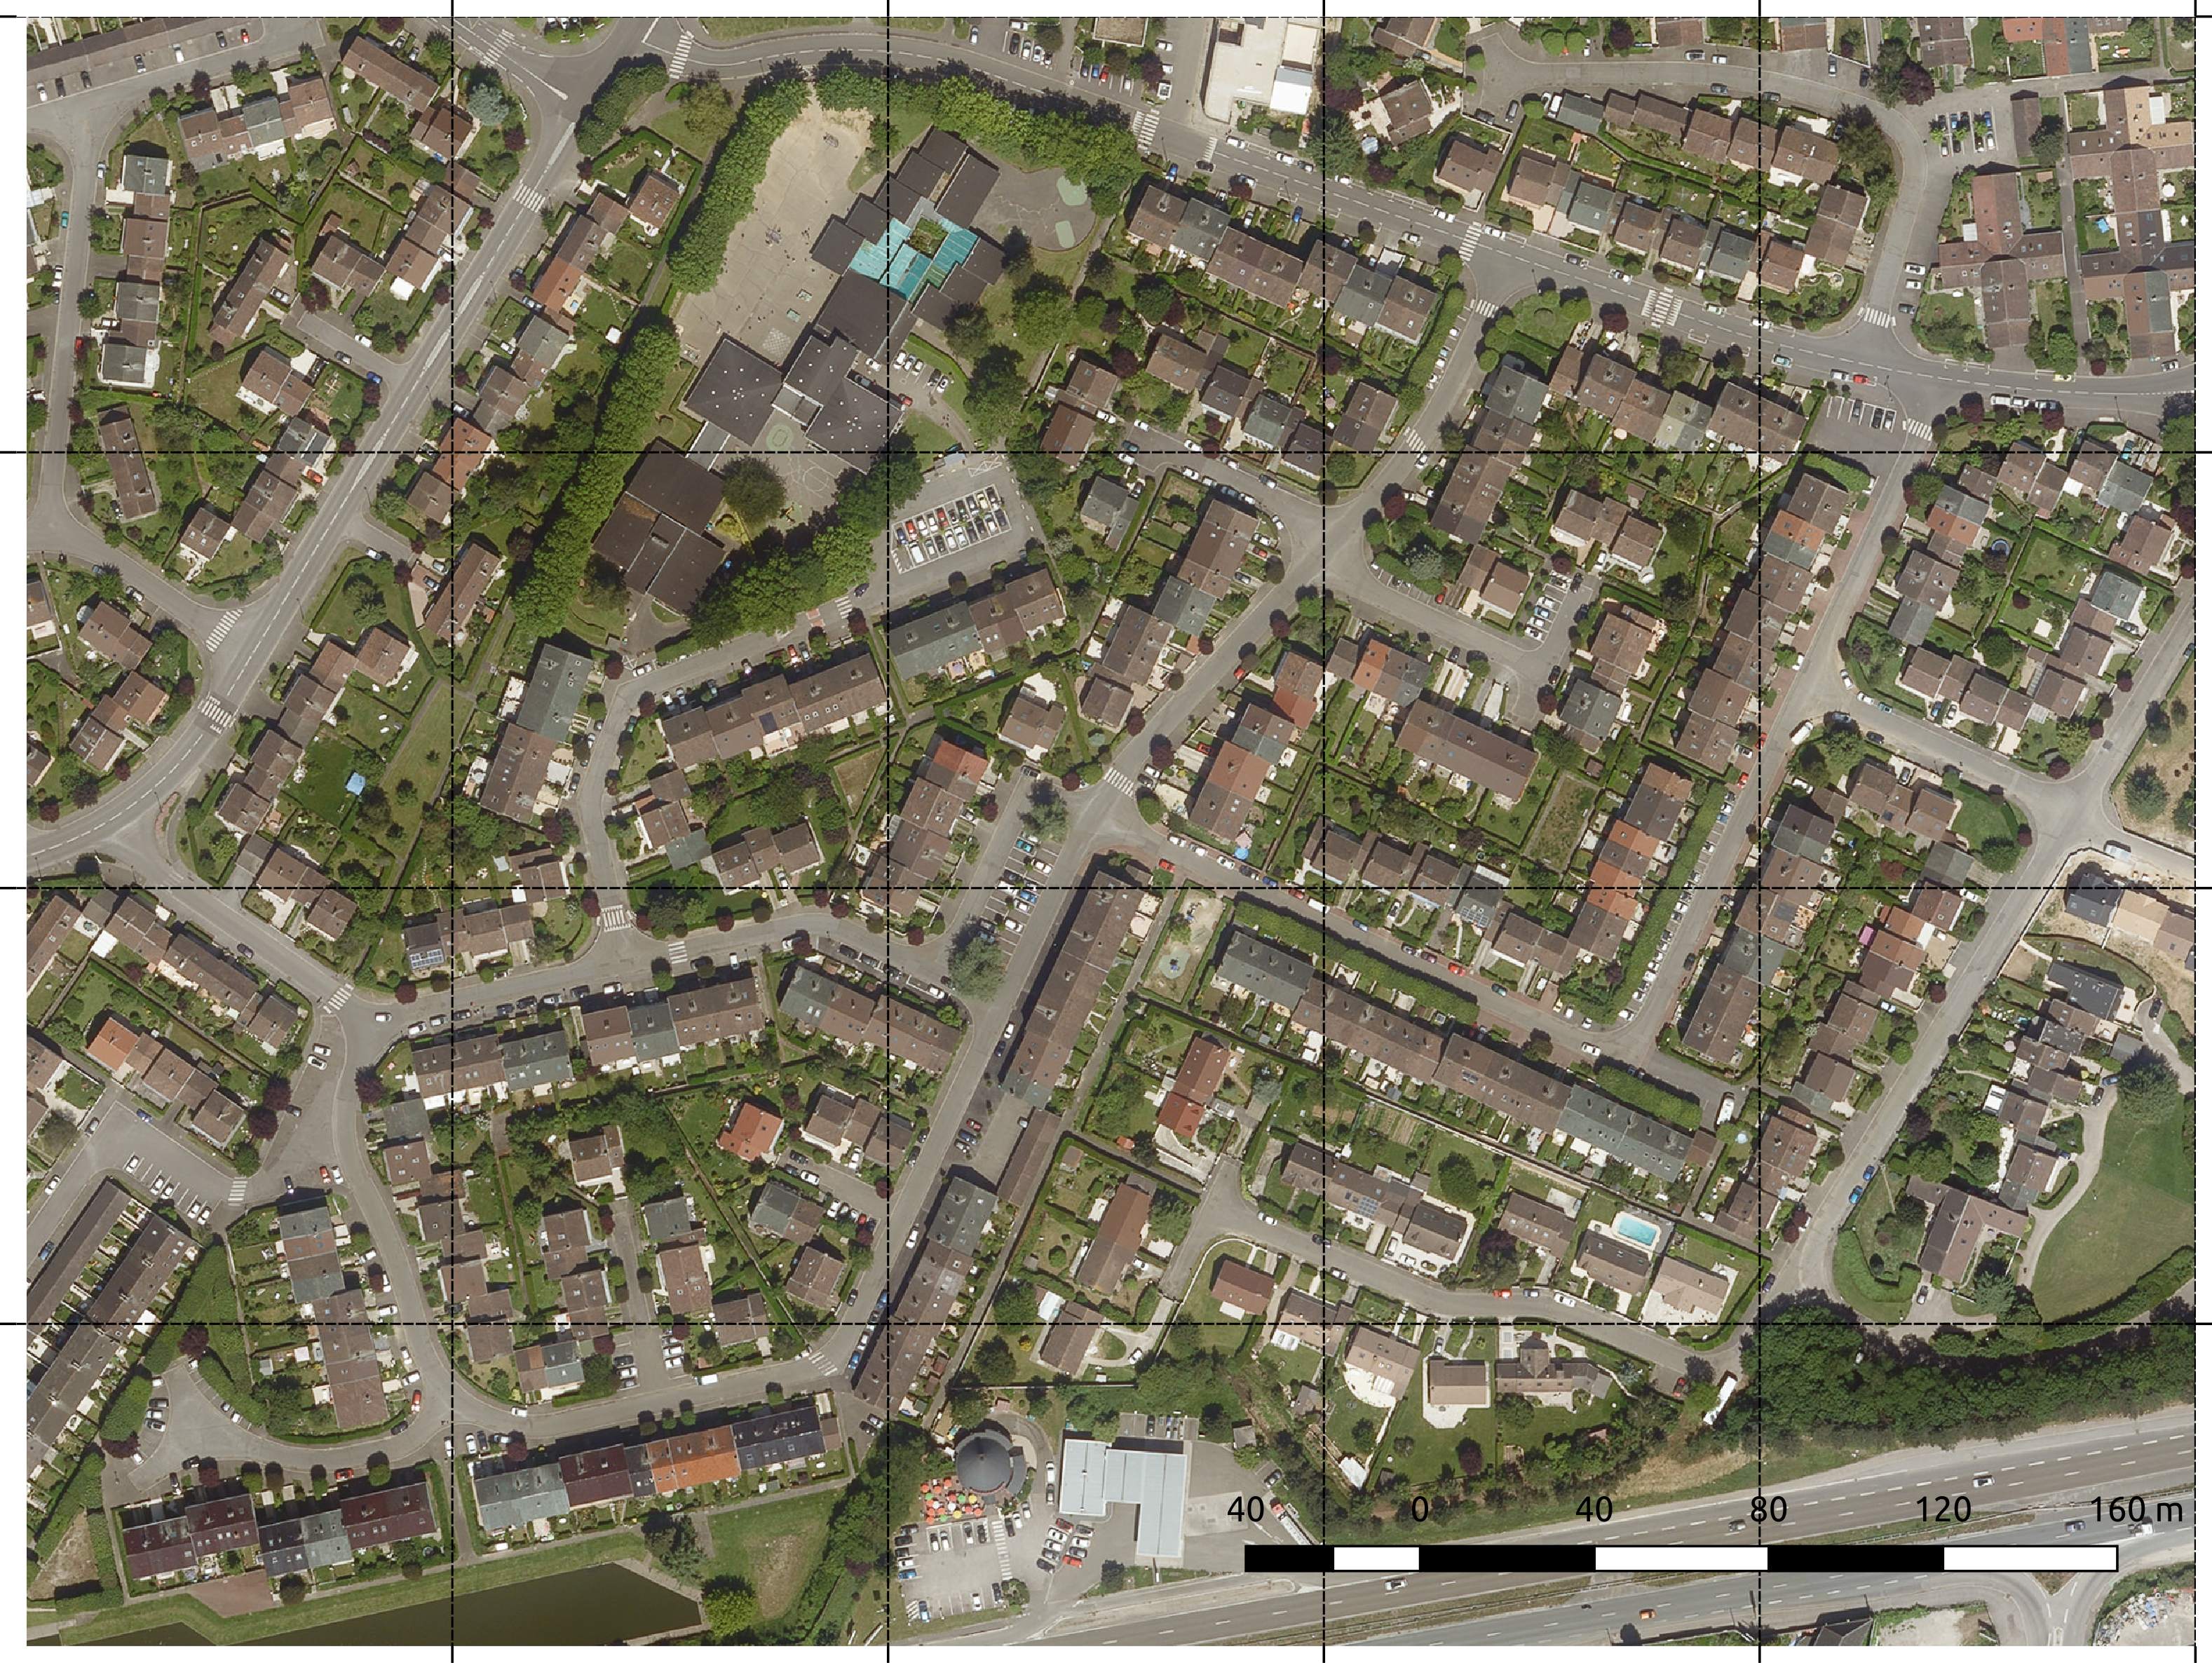
\includegraphics[width=.40\textwidth]{../images/raster/orthoimage}
                }
                {
                    \caption{Orthoimage corresponding to the scene.}\label{fig::ortho}
                }
                \ffigbox[\FBwidth]
                {
                    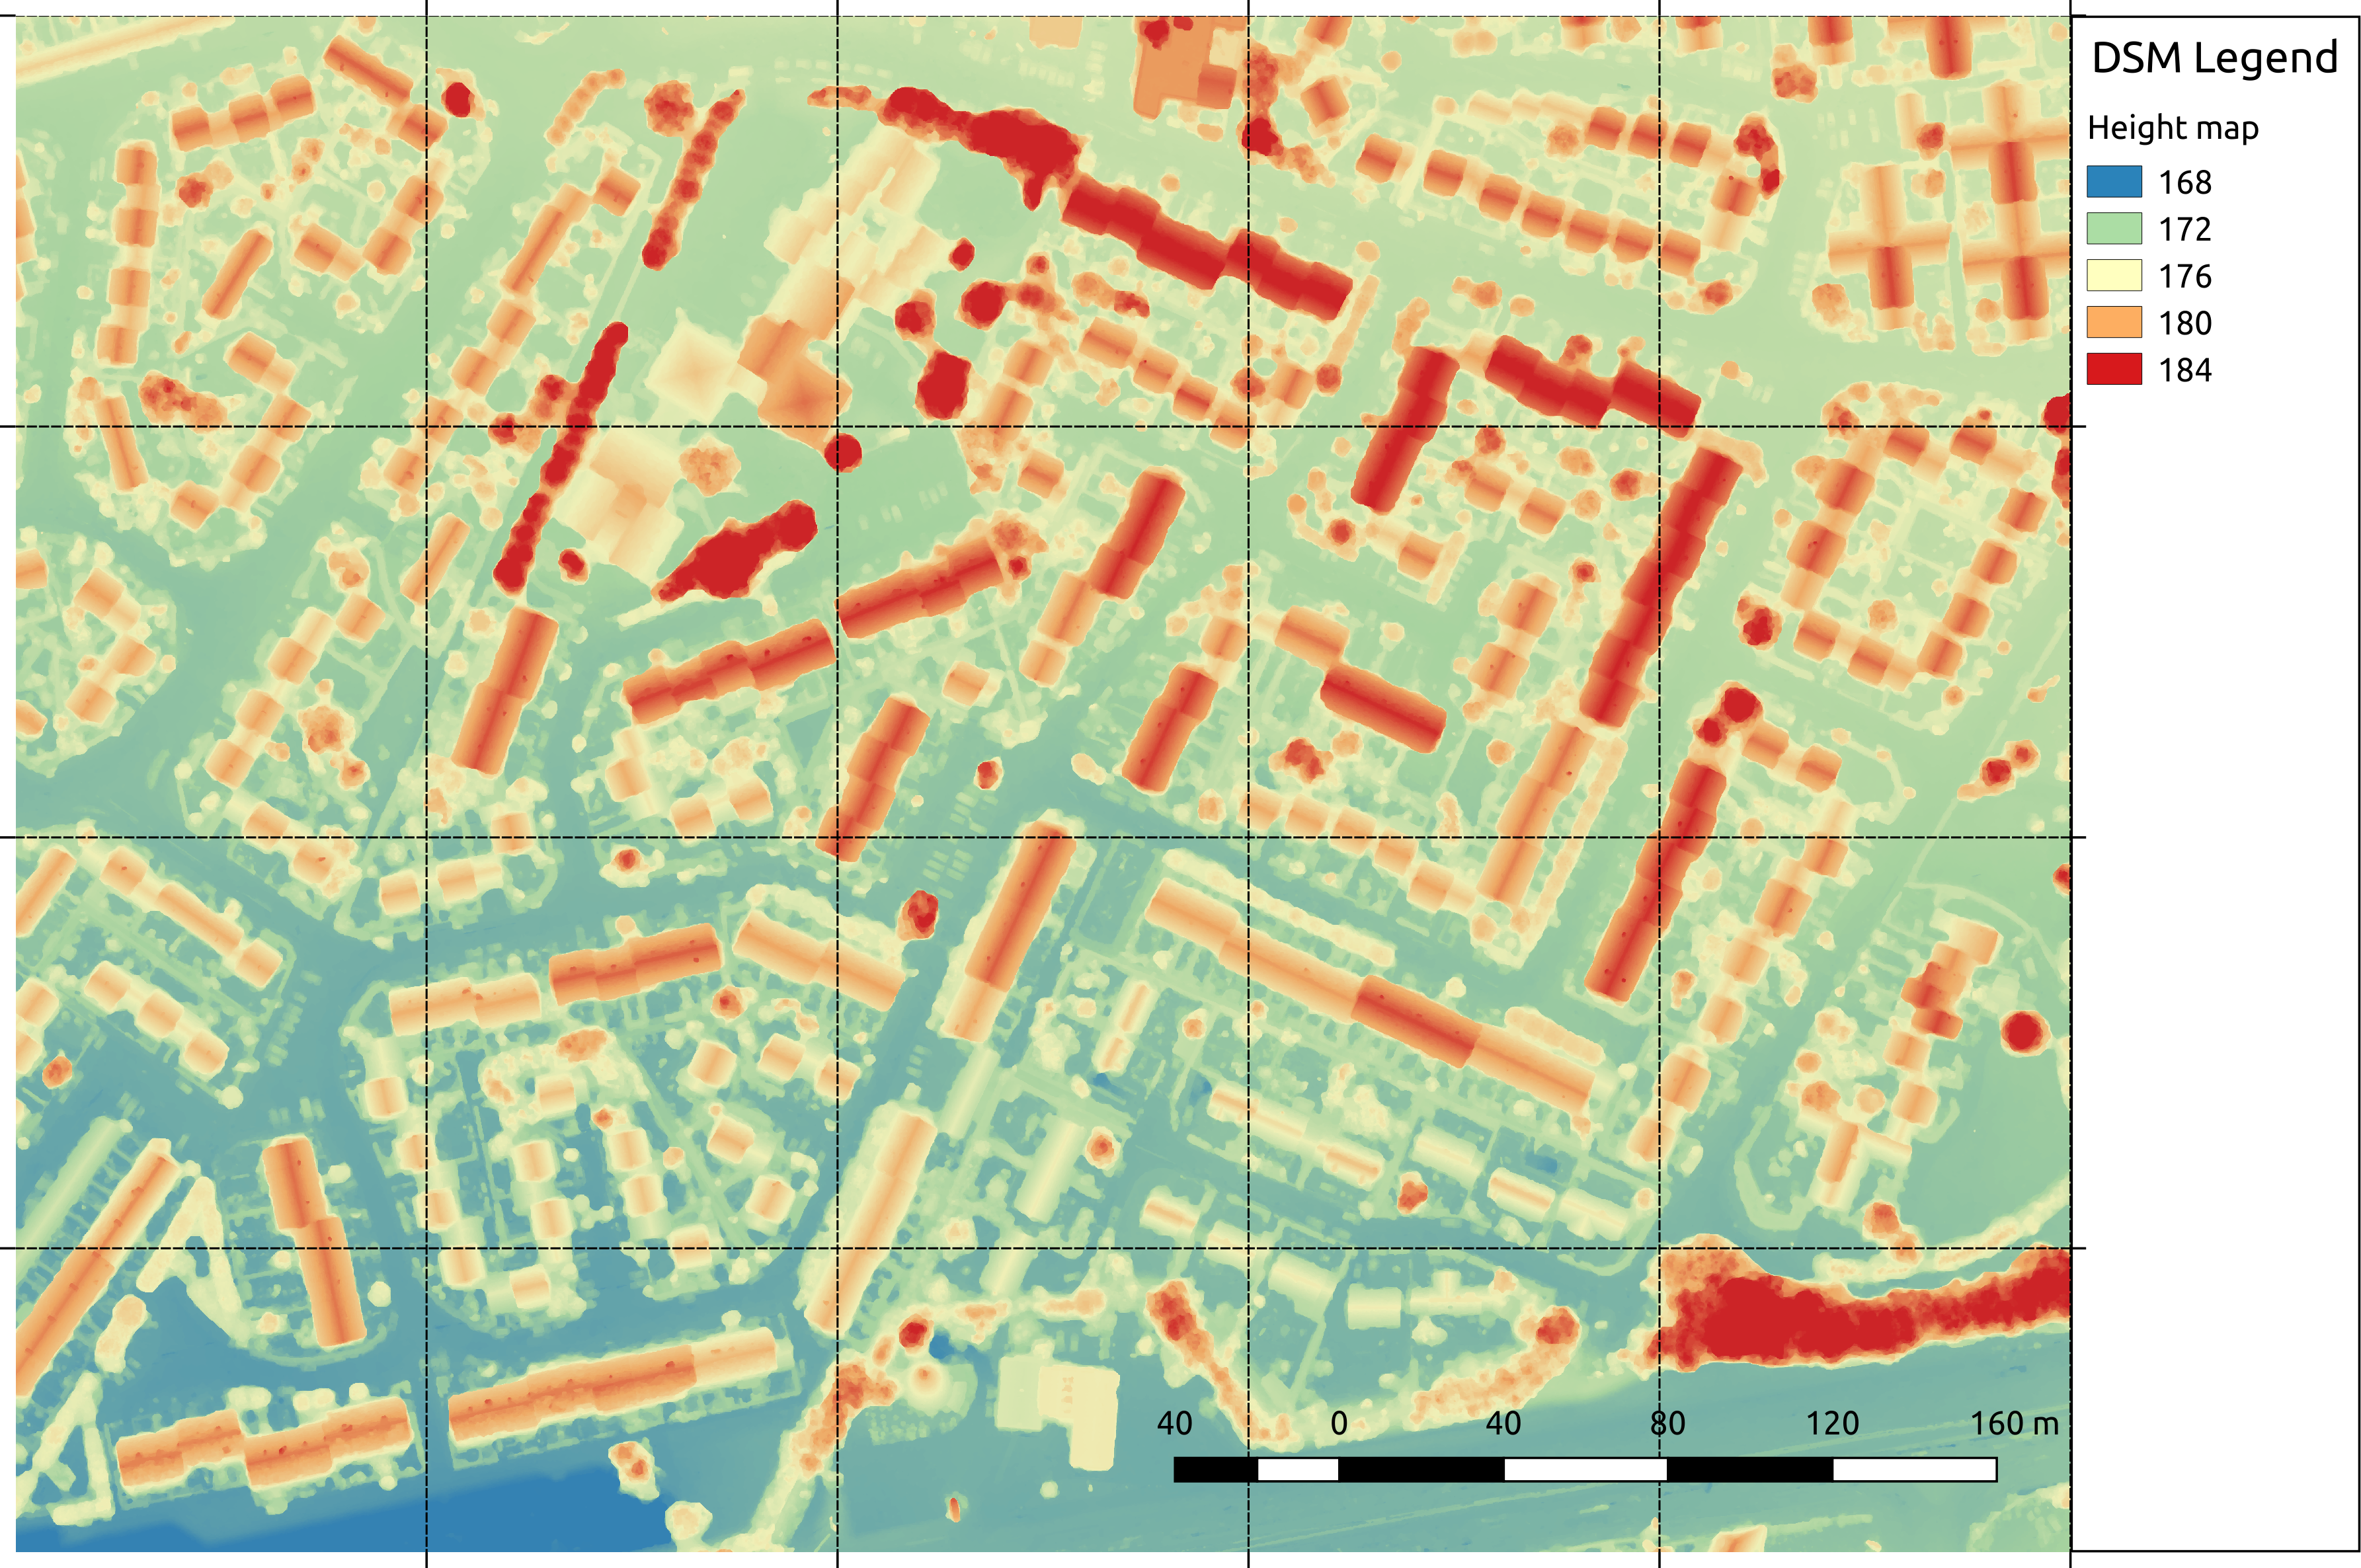
\includegraphics[width=.46\textwidth]{../images/raster/dsm}
                }
                {
                    \caption{.}\label{fig::dsm}
                }
            \end{subfloatrow}
        }
        {
            \caption{\label{fig::dataset} Data used in the qualification process.}
        }
    \end{figure}

    \subsection{Annotated errors}

    The taxonomy has evolved from the one proposed in earlier work~\cite{michelin2013quality}. The high level --- LoD based --- discrimination matured during the manual annotation into three metaclasses. Each one of these metaclasses is itself subdivided into errors. The errors are chosen to represent atomic flaws, in order to keep the taxonomy stable enough in case we expand to other regions. In fact, in case we stumble upon new cases we can feed each metaclass by corresponding erros. Multiple errors can alter a single building. The metaclasses are chosen to correlate to LoD levels: we estimate that this reprentation will not evolve further in the future.

    We proceed now to descibing, in full detail, these classes:

    \begin{enumerate}[(i)]
        \item Unqualified Building Errors (\textit{c.f.} Figure~\ref{fig::samples}\ref{fig::unq_bul}): buildings will not be taken into consideration, since we know before hand that they are not taken into account by the reconstruction method:
        \item Building Errors (\textit{c.f.} Figure~\ref{fig::samples}\ref{fig::bul_err}): encompasses the errors that affect the whole building (corrensponds roughly to $LoD0$ and $LoD1$ errors),
        \item Facet Errors (\textit{c.f.} Figure~\ref{fig::samples}\ref{fig::fac_err}): concerns errors affecting only a facet.
    \end{enumerate}

    The errors are summarized into a mindmap --- \textit{c.f.} Figure~\ref{fig::mindmap_errors}.

    \begin{sidewaysfigure}[p]
        \begin{center}
            \includestandalone[mode=buildnew, scale=.78]{mind_map}
            \caption{\label{fig::mindmap_errors} Mind map summarizing the errors encountered during annotation.}
        \end{center}
    \end{sidewaysfigure}

    In Table~\ref{tab::label_stats} we present some statistics over the labelled dataset (\textit{c.f.} Figure~\ref{fig::dataset}) comprizing $502$ buildings:

    \begin{sidewaystable}[H]
        \centering
        \caption{\label{tab::label_stats} Label statistics over the $502$ building dataset.}
        \begin{tabular}{x{4cm} | x{3cm} | x{3cm} | x{3cm} | x{3cm}}
            \toprule
            \multicolumn{1}{c|}{\textbf{Error Class}} & \textbf{Occurence probability} & \textbf{Subclass} & \textbf{Class conditionnal occurence probability} & \textbf{Absolute occurence probability} \\
            \midrule
            \multirow{4}{*}{Unqualified Buildings} & \multirow{4}{*}{$0.0876$} & Half Building & $0.8636$ & $0.0757$ \\
            \cline{3-5}
                &                   & Changed Building & $0.0455$ & $0.0040$ \\
            \cline{3-5}
                &                   & Occlusion & $0.0455$ & $0.0040$ \\
            \cline{3-5}
                &                   & Unknown & $0.0455$ & $0.0040$ \\
            \midrule
            \midrule
            \multirow{4}{*}{Building Error} & \multirow{4}{*}{$0.2408$} & Over Segmentation & $0.1365$ & $0.0328$\\
            \cline{3-5}
                &                   & Under Segmentation & $0.4177$ & $0.1006$ \\
            \cline{3-5}
                &                   & Footprint & $0.4839$ & $0.1165$ \\
            \cline{3-5}
                &                   & Altimetric & $0.0165$ & $0.0040$ \\
            \midrule
            \midrule
            \multirow{4}{*}{Facet Errors} & \multirow{4}{*}{$0.81657$} & Over Segmentation & $0.8830$ & $0.7203$ \\
            \cline{3-5}
                &                   & Under Segmentation & $0.0842$ & $0.0687$ \\
            \cline{3-5}
                &                   & Mis Segmentation & $0.0806$ & $0.0657$ \\
            \cline{3-5}
                &                   & Slope & $0.0327$ & $0.0267$ \\
            \bottomrule
        \end{tabular}
    \end{sidewaystable}

    \thisfloatsetup{heightadjust=object}
    \begin{figure}[H]
        \begin{center}
            \ffigbox{
                \ffigbox[\FBwidth]{
                    \begin{subfloatrow}[4]
                        \captionsetup{labelformat=brace, justification=raggedright}
                        \ffigbox[\FBwidth]{\caption{Half Building: only a portion of the building is reconstructed.}\label{fig::half_building}}{\fbox{\includegraphics[width=.24\textwidth]{../images/raster/Unqualified_Errors/half_building}}}
                        \ffigbox[\FBwidth]{\caption{Changed Building: the building has changed so we cannot qualify it.}\label{fig::changed}}{\fbox{\includegraphics[width=.24\textwidth]{../images/raster/Unqualified_Errors/changed}}}
                        \ffigbox[\FBwidth]{\caption{Occlusion: the building is occluded by vegetation here.}\label{fig::occlusion}}{\fbox{\includegraphics[width=.24\textwidth]{../images/raster/Unqualified_Errors/occlusion}}}
                        \ffigbox[\FBwidth]{\caption{Unknown: Unknown shape that cannot be verified on the ground.}\label{fig::unknown}}{\fbox{\includegraphics[width=.24\textwidth]{../images/raster/Unqualified_Errors/unknown}}}
                    \end{subfloatrow}
                }
                {
                    \renewcommand\figurename{}
                    \renewcommand{\thefigure}{(\roman{SubFigCounter})}

                    \caption{Unqualified building errors samples.}\label{fig::unq_bul}
                    \refstepcounter{SubFigCounter}
                }
                \ffigbox[\FBwidth]
                {
                    \begin{subfloatrow}[4]
                        \captionsetup{labelformat=brace, justification=raggedright}
                        \ffigbox[\FBwidth]{\caption{Under Segmentation: Two or more buildings grouped into one.}\label{fig::under_bul}}{\fbox{\includegraphics[width=.24\textwidth]{../images/raster/Building_Errors/under_segmentation}}}
                        \ffigbox[\FBwidth]{\caption{Over segmentation: One building segmented into two or more buildings.}\label{fig::over_bul}}{\fbox{\includegraphics[width=.24\textwidth]{../images/raster/Building_Errors/over_segmentation}}}
                        \ffigbox[\FBwidth]{\caption{Footprint: Wrong building footprint.}\label{fig::footprint}}{\fbox{\includegraphics[width=.24\textwidth]{../images/raster/Building_Errors/footprint}}}
                        \ffigbox[\FBwidth]{\caption{Altitude: Wrong building height.}\label{fig::too_low}}{\fbox{\includegraphics[width=.24\textwidth]{../images/raster/Building_Errors/altimetric}}}
                    \end{subfloatrow}
                }
                {
                    \renewcommand\figurename{}
                    \renewcommand{\thefigure}{(\roman{SubFigCounter})}

                    \caption{Building errors samples.}\label{fig::bul_err}
                    \refstepcounter{SubFigCounter}
                }
                \ffigbox[\FBwidth]
                {
                    \begin{subfloatrow}[4]
                        \captionsetup{labelformat=brace, justification=raggedright}
                        \ffigbox[\FBwidth]{\caption{Under Segmentation: Two facets or more grouped into one.}\label{fig::under_fac}}{\fbox{\includegraphics[width=.24\textwidth]{../images/raster/Facet_Errors/under_segmentation}}}
                        \ffigbox[\FBwidth]{\caption{Over segmentation: One facet segemented into two or more facets.}\label{fig::over_fac}}{\fbox{\includegraphics[width=.24\textwidth]{../images/raster/Facet_Errors/over_segmentation}}}
                        \ffigbox[\FBwidth]{\caption{Mis Segmentation: Facet edges do not correspond to real ones.}\label{fig::mis}}{\fbox{\includegraphics[width=.24\textwidth]{../images/raster/Facet_Errors/mis_segmentation}}}
                        \ffigbox[\FBwidth]{\caption{Slope: Wrong facet slope.}\label{fig::slope}}{\fbox{\includegraphics[width=.24\textwidth]{../images/raster/Facet_Errors/slope}}}
                    \end{subfloatrow}
                }
                {
                    \renewcommand\figurename{}
                    \renewcommand{\thefigure}{(\roman{SubFigCounter})}

                    \caption{Facet errors samples.}\label{fig::fac_err}
                    \refstepcounter{SubFigCounter}
                }
            }
            {
                \addtocounter{figure}{-3}
                \caption{\label{fig::samples}Error taxonomy illustration.}
            }
        \end{center}
    \end{figure}
\end{document}
